\subsection{Musculoskeletal Model Wrapper}
\label{sec:impl_opensim}

This subsection describes the implementation of the \texttt{OpenSimComponent} backend wrapper class. It addresses requirement SR-03-02 (integration of musculoskeletal simulation tools) by mapping OpenSim models onto the \texttt{CoSimComponent} interface defined in Section~\ref{sec:impl_component_interface}.
The wrapper delegates all multibody and muscle dynamics to the OpenSim library, which itself builds on the Simbody multibody engine, and encapsulates the realize-integrate cycle behind the primitive and hook operations of the component contract.

% --- BACKGROUND BRIDGE ---
As introduced in Section~\ref{sec:theory_opensim}, an OpenSim model is a Simbody multibody system whose state is advanced by an integrator driven through an \texttt{osim.Manager}.
All derived quantities, such as body positions, forces, muscle activations, generalized accelerations, are obtained from the state through staged realization (\textit{Position},
\textit{Velocity}, \textit{Dynamics}, \textit{Acceleration}).
The wrapper does not re-implement any of this machinery.
Its role is to present an OpenSim model as a \syssimx{} component whose ports, parameters, and lifecycle are aligned with the rest of the framework.

%%%%%%%%%%%%%%%%%%%%%%%%%%%%%%%%%%%%%%%%%%%%%%%%%%%%%%
\subsubsection{Architecture and Interface Mapping}

Figure~\ref{fig:impl_opensim_class} shows the class-level relationship between \texttt{OpenSimComponent}, its abstract base \texttt{CoSimComponent}, and the external OpenSim objects \texttt{Model}, \texttt{Manager}, and \texttt{State}.
Unlike \texttt{FMUComponent} (Section~\ref{sec:impl_fmu}), \texttt{OpenSimComponent} is itself an \emph{abstract base} since OpenSim models do not expose a standardized interface descriptor analogous to \texttt{modelDescription.xml}, so ports, parameters, and the model-assembly steps must be declared by a concrete subclass that targets a specific musculoskeletal model.
The base class provides the infrastructure that is common to every OpenSim component.

\begin{figure}[htbp]
  \centering
  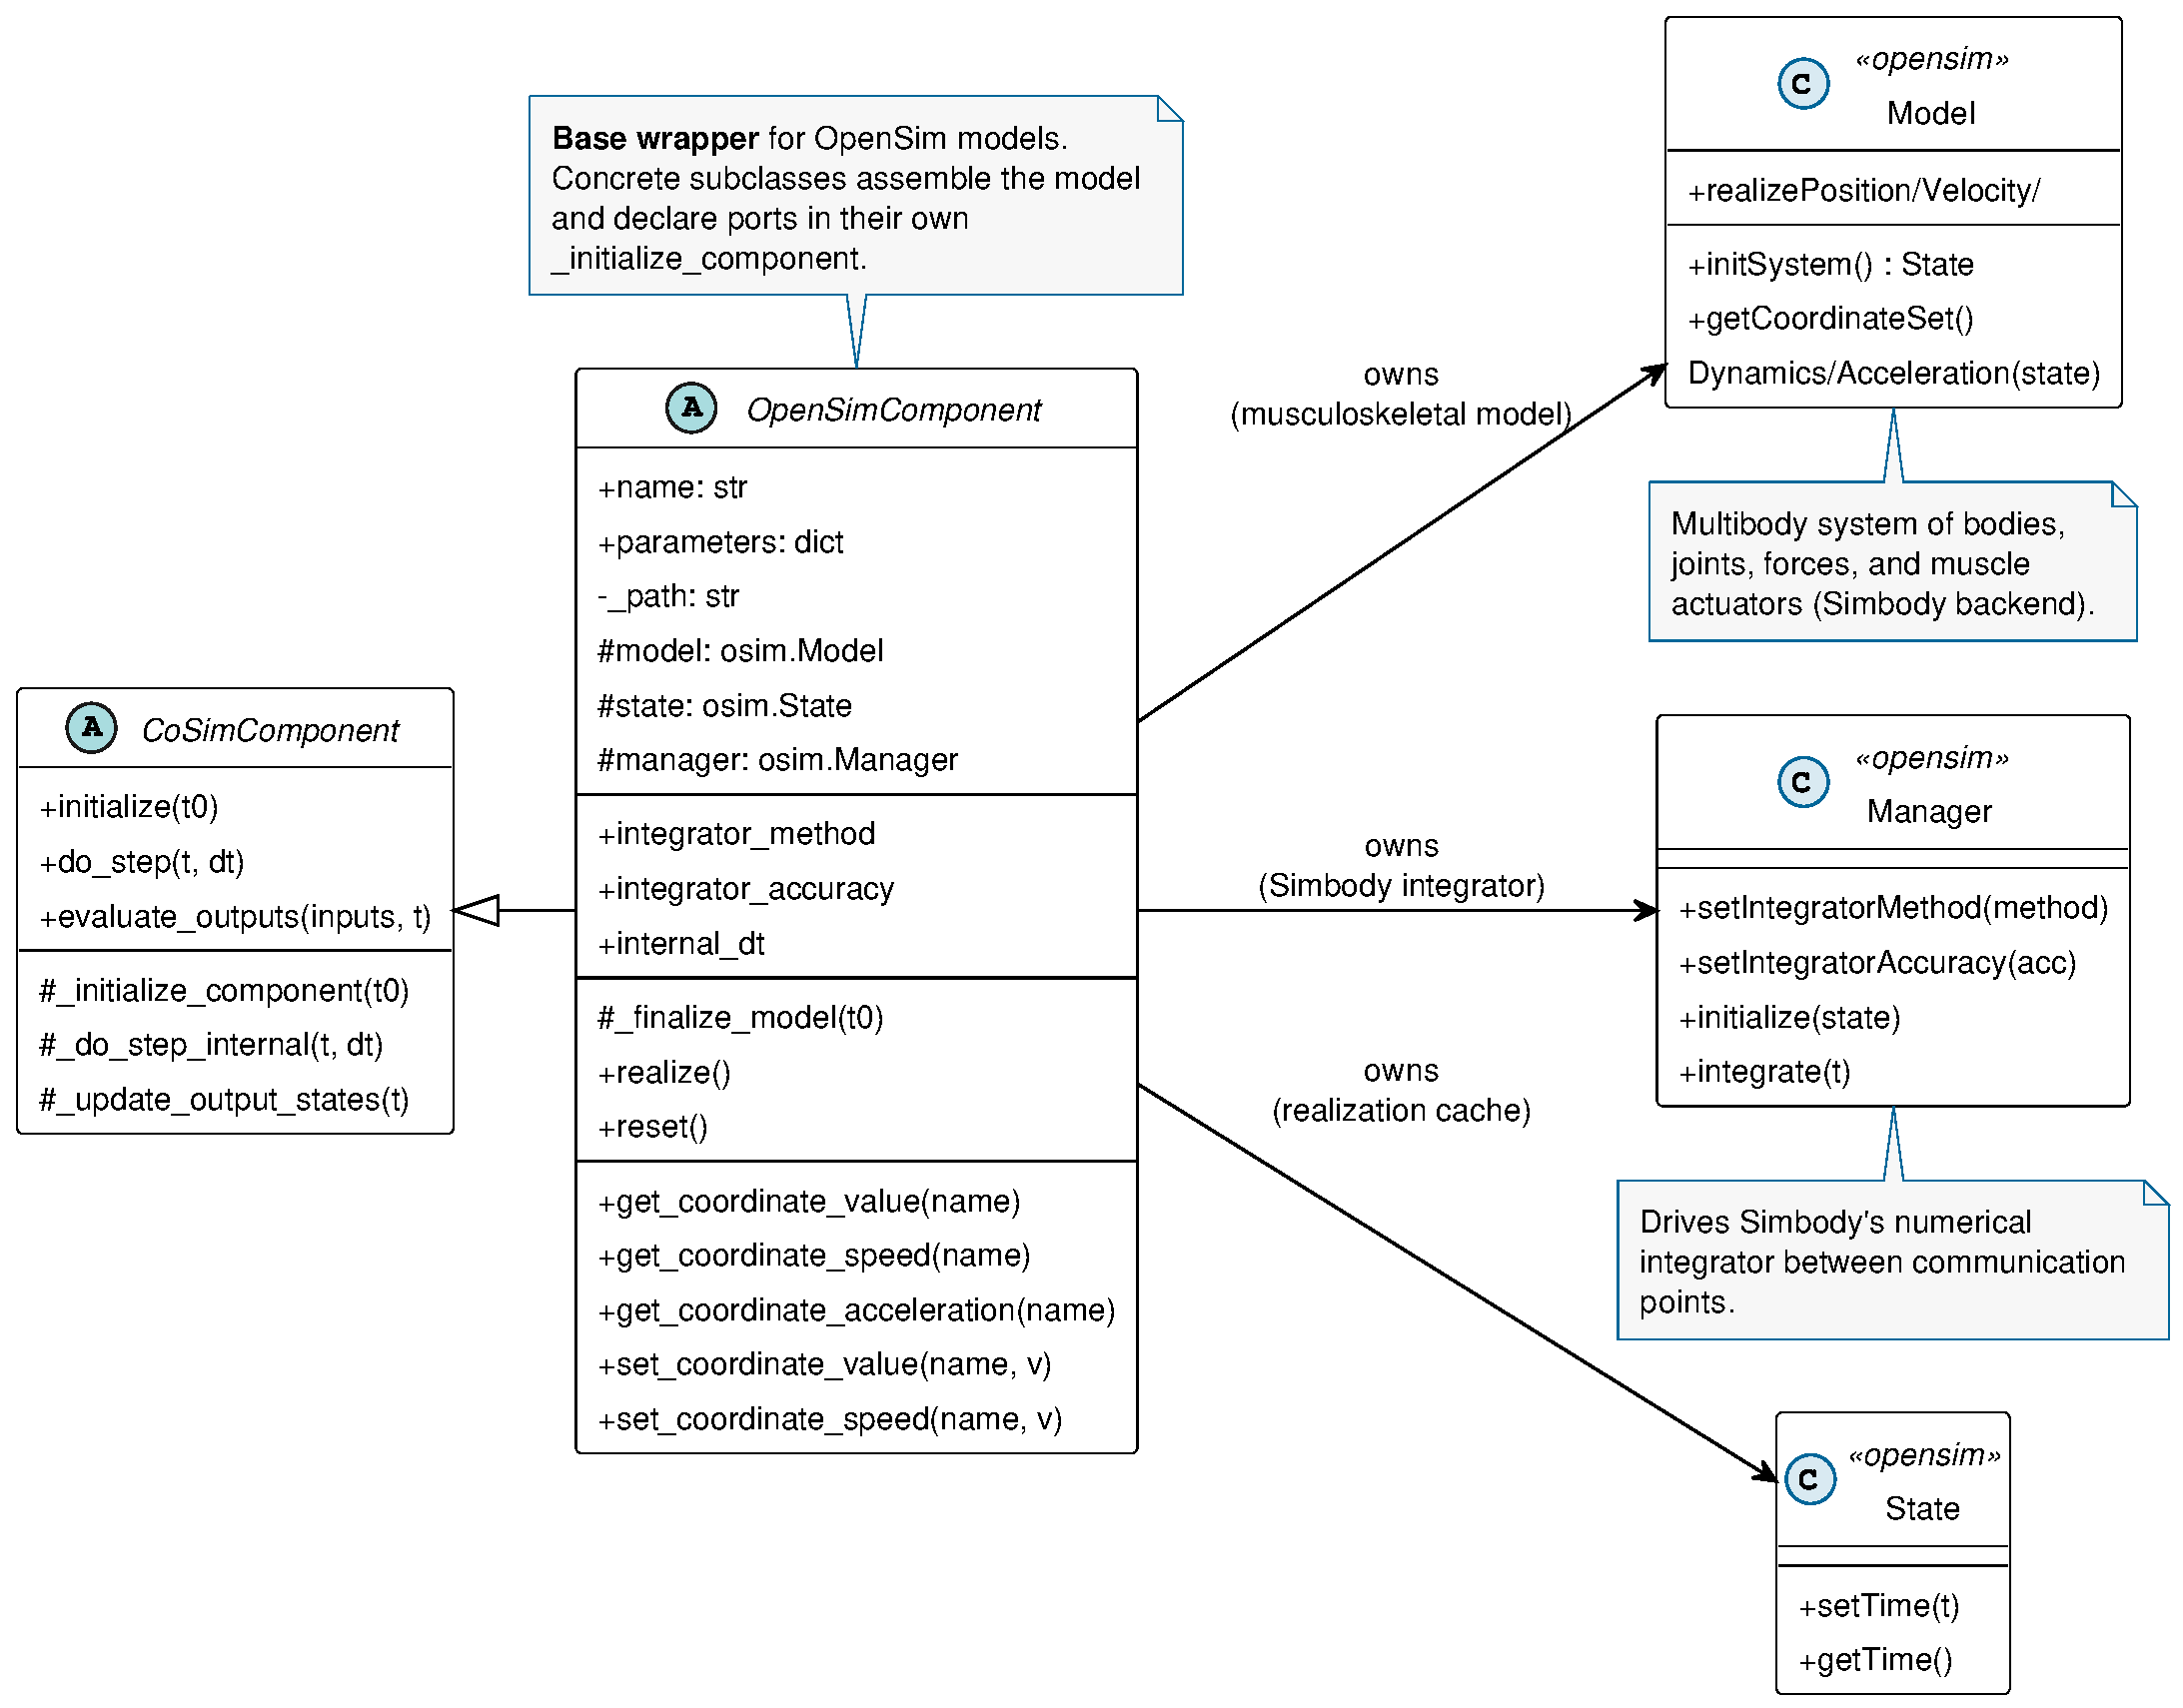
\includegraphics[width=\linewidth]{diagrams/out/pdf/class/components/OpenSimComponent.pdf}
  \caption{Class diagram of the OpenSim wrapper.
           \texttt{OpenSimComponent} specializes
           \texttt{CoSimComponent} and serves as an abstract base for
           concrete musculoskeletal components. It owns an
           \texttt{osim.Model} (multibody system of bodies, joints, forces,
           and muscles), an \texttt{osim.Manager} that drives Simbody's
           integrator, and the associated \texttt{osim.State} that holds
           time, generalized coordinates and velocities, and muscle
           states.}
  \label{fig:impl_opensim_class}
\end{figure}

\paragraph{OpenSim-to-Component Mapping.}
Table~\ref{tab:opensim_mapping} lists the correspondence between OpenSim artefacts and the component abstractions introduced in Sections~\ref{sec:impl_port_system} and \ref{sec:impl_component_interface}.
Unlike the FMU case, the mapping is authored once per concrete subclass rather than derived from a descriptor file.

\begin{table}[htbp]
  \centering
  \small
  \caption{Mapping between OpenSim artefacts and \syssimx{} component
           abstractions. The mapping is established by the concrete
           subclass during construction and initialization.}
  \label{tab:opensim_mapping}
  \begin{tabular}{p{6.3cm} p{7.5cm}}
    \toprule
    \textbf{OpenSim artefact} & \textbf{\syssimx{} abstraction} \\
    \midrule
    \texttt{osim.Model} loaded from a \texttt{.osim} file
      & Backend object owned by the concrete component \\
    \addlinespace
    Selected \texttt{Coordinate} values / speeds
      & \texttt{PortSpec} entries (direction \texttt{in}/\texttt{out}) \\
    \addlinespace
    Muscle activations, control signals, actuator excitations
      & Input \texttt{PortSpec} entries with dimensionless units \\
    \addlinespace
    Body kinematics, muscle forces, generalized accelerations
      & Output \texttt{PortSpec} entries with SI units \\
    \addlinespace
    Model properties set before \texttt{initSystem()}
      & Entries in the component's \texttt{parameters} dictionary \\
    \addlinespace
    Integrator method, accuracy, internal step size
      & Attributes \texttt{integrator\_method},
        \texttt{integrator\_accuracy}, \texttt{internal\_dt} \\
    \bottomrule
  \end{tabular}
\end{table}

\paragraph{Direct-Feedthrough Detection.}
OpenSim does not declare input--output dependencies in a machine-readable form.
\texttt{OpenSimComponent} therefore inherits the default perturbation-based detector from \texttt{CoSimComponent} (Section~\ref{sec:impl_component_interface}). In practice, musculoskeletal
components are almost never feedthrough at the port level as muscle excitations affect activations and forces through differential dynamics, so the corresponding outputs lag the inputs by at least one step.

%%%%%%%%%%%%%%%%%%%%%%%%%%%%%%%%%%%%%%%%%%%%%%%%%%%%%%
\subsubsection*{Lifecycle Realization}

The base class provides the skeleton of the lifecycle and delegates model-specific assembly to the subclass.

\paragraph{Initialization.}
A concrete \texttt{\_initialize\_component(t0)} typically performs the
following steps:
\begin{enumerate}[nosep]
  \item Load the \texttt{.osim} model from the stored path into
        \texttt{self.model}.
  \item Attach any actuators, controllers, or analyses required by the
        port specification.
  \item Apply parameter start values declared on the component.
  \item Call \texttt{self.model.initSystem()} to obtain the initial
        \texttt{osim.State}.
  \item Invoke the inherited helper \texttt{\_finalize\_model(t0)}.
\end{enumerate}
\texttt{\_finalize\_model(t0)} realizes the state through the \textit{Acceleration} stage, instantiates an \texttt{osim.Manager}, configures its integrator method and accuracy, calls \texttt{manager.initialize(state)}, and sets the simulation time to $t_0$.
After the template method \texttt{initialize()} returns, the initial outputs are available in the \texttt{PortState} objects and recorded in the component history.

\paragraph{Stepping.}
\texttt{\_do\_step\_internal(t, dt)} writes the current input ports into the OpenSim state (for example through \texttt{set\_coordinate\_value}/\texttt{set\_coordinate\_speed} or by assigning excitations to controllers) and then issues a single call to \texttt{self.manager.integrate($t+dt$)}. The Simbody integrator advances the state internally with its own adaptive step size, bounded by
\texttt{integrator\_accuracy}.
The communication step $dt$ only defines the boundary at which the coupled simulation synchronizes.

\paragraph{Output Refresh.}
\texttt{\_update\_output\_states()} first calls \texttt{realize()} to
bring the state to the \textit{Acceleration} stage and then reads the port-relevant quantities. Coordinate values, speeds, and accelerations are obtained through the name-based helpers \texttt{get\_coordinate\_value}, \texttt{get\_coordinate\_speed}, and \texttt{get\_coordinate\_acceleration}; muscle and actuator quantities are obtained through the corresponding OpenSim accessor calls.
The results are written back into the \texttt{PortState} objects with their declared units.

\paragraph{Coordinate Helpers.}
The helpers \texttt{get\_coordinate\_*} and \texttt{set\_coordinate\_*} abstract over the \texttt{CoordinateSet} lookup that OpenSim requires for every access and are used by every concrete subclass.
They also serve as the state-transfer primitives used in the multi-model switching
mechanism (Section~\ref{sec:impl_multi_model}), where generalized positions and velocities must be copied between backends whose state representations otherwise differ.

%%%%%%%%%%%%%%%%%%%%%%%%%%%%%%%%%%%%%%%%%%%%%%%%%%%%%%
\subsubsection*{State Access and Rollback Boundary}

The generic \texttt{OpenSimComponent} exposes \texttt{get\_state()} and \texttt{set\_state()} in the same sense as \texttt{FMUComponent}: as a readable dictionary of generalized coordinates, speeds, and activations together with their declared units.
This dictionary is intended for inspection, state transfer across components, and re-initialization.It is not an opaque snapshot of the Simbody integrator.

The method \texttt{reset()} releases the existing \texttt{osim.State} and \texttt{osim.Manager} and re-creates them from the current \texttt{osim.Model}, so that the component can be reinitialized for a new run.
The generic base class does not override \texttt{snapshot\_state()} or \texttt{restore\_state()}; rollback for the hybrid algorithm is implemented only in specialized subclasses whose concrete model and integrator make state restoration well defined.

%%%%%%%%%%%%%%%%%%%%%%%%%%%%%%%%%%%%%%%%%%%%%%%%%%%%%%
\subsubsection*{Verification}

Because \texttt{OpenSimComponent} is an abstract base, verification is performed through a minimal concrete subclass that wraps a simple single-degree-of-freedom pendulum model (one body, one pin joint, one torque actuator).
Table~\ref{tab:opensim_verification} lists the verified properties.

\begin{table}[htbp]
  \centering
  \small
  \caption{Verified properties of \texttt{OpenSimComponent}. All tests
           use a minimal single-degree-of-freedom pendulum model driven
           by a coordinate actuator.}
  \label{tab:opensim_verification}
  \begin{tabular}{p{6.5cm} p{7.5cm}}
    \toprule
    \textbf{Verified property} & \textbf{Expected outcome} \\
    \midrule
    Model loading and system initialization
      & \texttt{initSystem()} produces a valid \texttt{State} realized to
        the \textit{Acceleration} stage after
        \texttt{\_finalize\_model(t0)} \\
    \addlinespace
    Coordinate helpers
      & \texttt{get\_/set\_coordinate\_value/speed} apply to and read
        from the \texttt{osim.State} consistently and respect unit
        declarations \\
    \addlinespace
    Parameter application
      & Values assigned through \texttt{set\_parameters()} are reflected
        in the model before \texttt{initSystem()} is called \\
    \addlinespace
    Integrator configuration
      & The chosen \texttt{integrator\_method} and
        \texttt{integrator\_accuracy} are applied to the
        \texttt{osim.Manager} used for stepping \\
    \addlinespace
    Initialize--step--reset cycle
      & Full lifecycle completes without resource leaks; the component
        is reusable after \texttt{reset()} \\
    \addlinespace
    Energy behaviour of the pendulum
      & For an unactuated swing over a short horizon, total mechanical
        energy drifts within the tolerance implied by
        \texttt{integrator\_accuracy} \\
    \addlinespace
    State serialization
      & \texttt{get\_state()} returns the generalized coordinates,
        speeds, and declared parameters with units; \texttt{set\_state()}
        restores them into a freshly reset component \\
    \bottomrule
  \end{tabular}
\end{table}

These properties confirm that \texttt{OpenSimComponent} faithfully adapts the OpenSim realize--integrate cycle to the component contract without leaking backend-specific semantics.
The integration with the FMI control stack and the FEM-based contact element of the controlled pendulum is deferred to the case study in Chapter~\ref{chap:case_study}.